%%%% CAPÍTULO 3 - MATERIAL E MÉTODOS (PODE SER OUTRO TÍTULO DE ACORDO COM O TRABALHO REALIZADO)

\chapter{Metodologia}\label{cap:materialemetodos}

O projeto foi estruturado em duas etapas principais: o desenvolvimento da
infraestrutura de \textit{hardware} e a criação do \textit{software}.
Além da criação do protótipo físico, foi elaborado um código com o 
objetivo de alcançar desempenho otimizado, atendendo a todos os 
requisitos do projeto. Isso incluiu desde a fase inicial de inicialização 
até a implementação de uma interface gráfica para os usuários, a entrada 
de dados, o reconhecimento facial, o cadastro e exclusão de usuários, 
por fim, o módulo de acionamento.

O fluxograma apresentado na \autoref{fig:fluxoprog} oferece uma visão
simplificada do funcionamento do \textit{software} do projeto. O sistema
de controle de acesso por biometria facial opera em dois ciclos principais:
o primeiro é dedicado à autenticação do usuário, enquanto o segundo é responsável
pelo cadastro de usuários. Além disso, há um ciclo obrigatório com um
temporizador em execução em segundo plano. Esse ciclo é ativado
automaticamente sempre que um dos ciclos principais é iniciado, com o intuito
de encerrar quaisquer atividades pendentes e prevenir possíveis \textit{loops}
dentro do sistema.

\begin{figure}[h!]
    \centering
    \caption{Fluxograma do \textit{firmware}}
    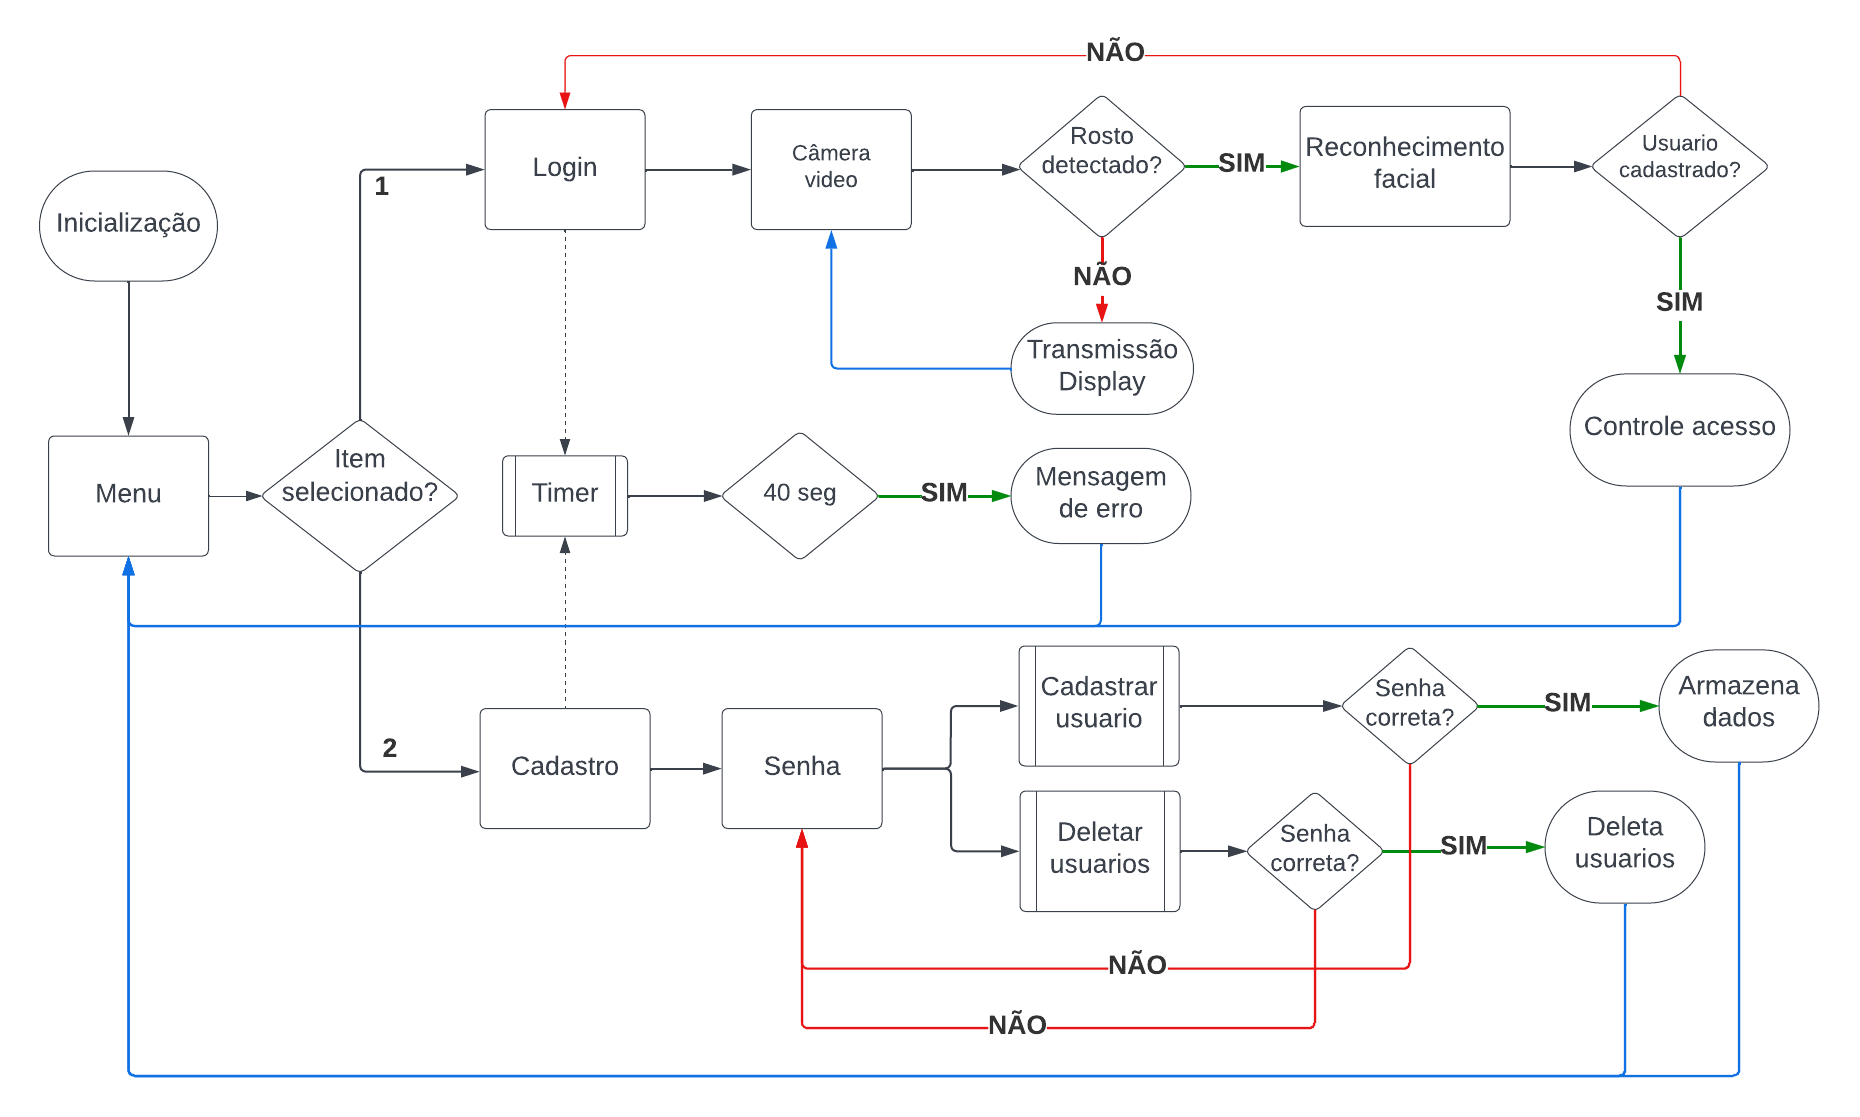
\includegraphics[scale=0.25]{figuras/fluxo_app.png}
    \fonte{}%% Fonte
    \label{fig:fluxoprog}
    \centering
\end{figure}

Para a execução desse programa, é necessário o uso de um \textit{hardware}
capaz de processá-lo. Portanto, a primeira etapa do projeto foi dedicada à
construção do protótipo físico. E com o intuito de facilitar a compreensão desta
parte do projeto, foi criado o diagrama apresentado na \autoref{fig:fluxohard}.
Conforme evidenciado, o ESP32-CAM é o módulo central, encarregado do
processamento de dados e da coordenação das informações aos demais módulos.
Para melhorar a interação com os usuários, é adicionado o módulo com botões e
uma interface gráfica (\textit{display}). Por fim, o módulo relé é
responsável pelo controle de acesso, podendo acionar diferentes tipos de
fechaduras elétricas.

\begin{figure}[h!]
    \centering
    \caption{Diagrama de blocos do \textit{hardware}}
    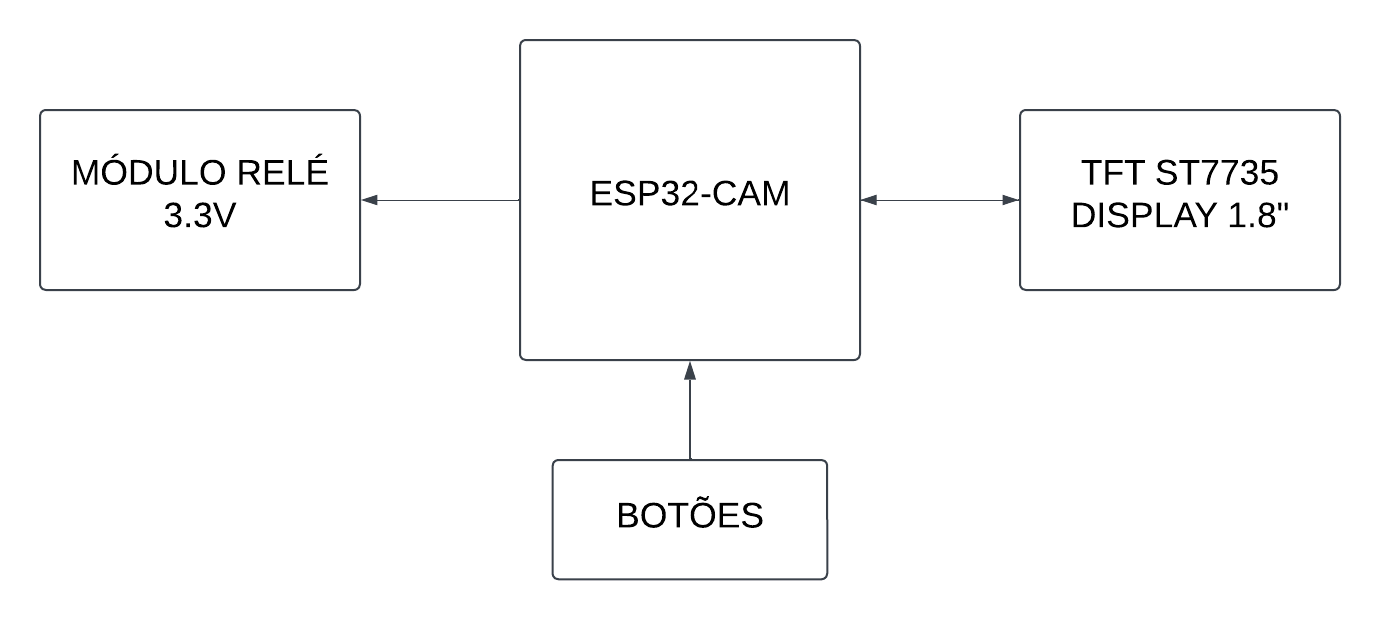
\includegraphics[scale=0.22]{figuras/diagrama_hardware.png}
    \fonte{}%% Fonte
    \label{fig:fluxohard}
    \centering
\end{figure}

Como um dos objetivos do projeto é o desenvolvimento de um protótipo de
baixo custo, a versão selecionada para essa finalidade é o ESP32-CAM,
que se destaca por integrar um \textit{chip} ESP32, uma câmera, uma
entrada para cartão SD e LED de alto brilho.

\section{Microcontrolador ESP32-CAM}\label{sec:materiais}

O ESP32-CAM (conforme ilustrado na \autoref{fig:espcam}) é um
microcontrolador desenvolvido pela empresa
\textit{Espressif Systems}® e que se destaca pelo seu custo beneficio.
Embora compacto, foi uma escolha ideal para este projeto devido à sua
variedade de recursos. Seu \textit{chip} é o ESP32-S, possui uma câmera integrada 
à placa, um processador \textit{Xtensa® dual-core} LX6 de 32 bits, um \textit{clock} 
ajustável com uma frequência máxima de 240MHz, 4 MB de memória 
\textit{Flash} e disponibiliza 16 pinos de Entrada/Saída (E/S), como 
pode ser visto no esquemático do Apêndice \ref{cap:apendiceb}.

Neste projeto, o ESP32-CAM desempenhou um papel central, sendo
responsável pelo processamento de dados, análise das informações
e controle dos demais componentes de \textit{hardware}. Isso incluiu
o gerenciamento de dispositivos adicionais e a coordenação das funções
necessárias para a aplicação proposta.

\begin{figure}[h!]
    \centering
    \caption{ESP32-CAM}
    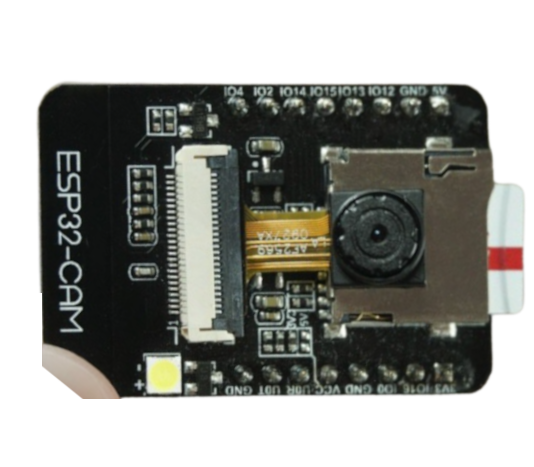
\includegraphics[scale=0.25]{figuras/esp32cam.png}
    \legend{Fonte: Adaptado de \citeonline{espcamimg}.}
    \label{fig:espcam}
    \centering
\end{figure}

\subsection{Pinos de Entrada/Saída (E/S)}\label{sec:gpio}

Os 16 pinos de Entrada/Saída (E/S) do ESP32-CAM (\autoref{fig:esp32pin})
desempenham um papel crucial na versatilidade
e funcionalidade deste microcontrolador.
Esses pinos oferecem uma interface flexível para conectar o
ESP32-CAM a uma ampla variedade de dispositivos e periféricos
externos, permitindo que ele interaja com o ambiente e execute
tarefas específicas de acordo com as necessidades do projeto.

\begin{figure}[h!]
    \centering
    \caption{GPIO disponíveis do ESP32-CAM}
    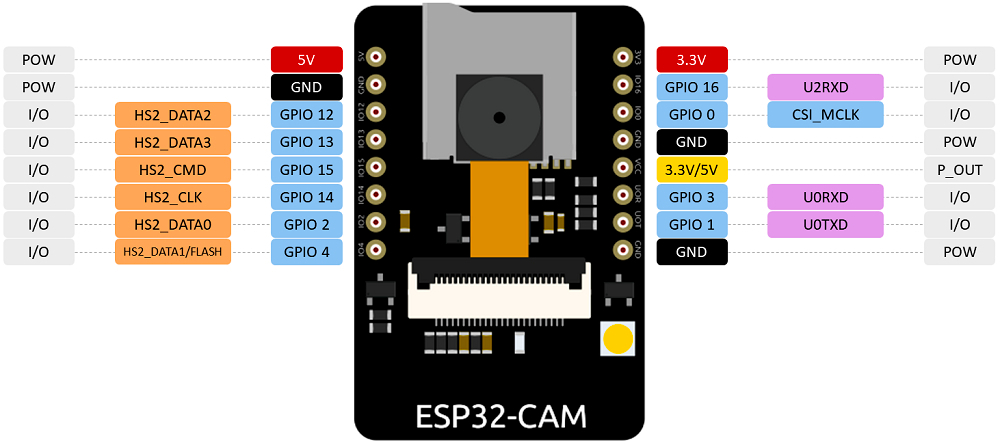
\includegraphics[scale=0.28]{figuras/esp32pin.jpg}
    \legend{Fonte: Adaptado de \citeonline{esp32pin}.}
    \label{fig:esp32pin}
    \centering
\end{figure}

Esses pinos são necessários para a comunicação com sensores, atuadores,
dispositivos de armazenamento, \textit{displays} e muitos outros componentes
eletrônicos, tornando o ESP32-CAM
adequado para inúmeras aplicações, desde sistemas de
segurança e monitoramento, até projetos de automação residencial.

No quadro a seguir (\autoref{quad:quadro1}), são detalhadas as funcionalidades dos 16 pinos 
de Entrada/Saída (E/S) disponíveis no ESP32-CAM. O entendimento destes pinos, possibilita 
aos desenvolvedores a flexibilidade de personalizar e expandir suas 
aplicações de acordo com suas necessidades específicas.

\begin{tabframed}[htb]
    \caption{Portas de Entrada/Saída ESP32-CAM}
    \label{quad:quadro1}
    \begin{tabular}{|l|l|}
        \hline
        \textbf{Pinos} & \textbf{Descrição}                                                                          \\ \hline
        5V             & Pino de entrada para alimentação do circuito do ESP32.                                      \\ \hline
        3GND           & 3 pinos de aterramento, usado para referência de potencial zero.                          \\ \hline
        GPIO12         & Pino de propósito geral.                                                                    \\ \hline
        GPIO13         & Pino de propósito geral.                                                                    \\ \hline
        GPIO15         & Pino de propósito geral.                                                                    \\ \hline
        GPIO14         & Pino de propósito geral.                                                                    \\ \hline
        GPIO2          & Pino de propósito geral.                                                                    \\ \hline
        GPIO4          & Pino de propósito geral e pode ser utilizado para acionar o Flash do ESP32.                 \\ \hline
        3.3V           & Pino de fornecimento de energia de 3,3V.                                                    \\ \hline
        GPIO16         & Este pino sempre fica em nível lógico alto e é utilizado para alimentar o circuto de PSRAM. \\ \hline
        GPIO0          & Pino de propósito geral, entretanto este pino é responsável pelo clock da câmera.           \\ \hline
        3.3V/5V        & Pode fornecer energia de 3,3V ou 5V para outros dispositivos.                               \\ \hline
        GPIO3          & Pino de entrada de dados UART (RX) para comunicação serial.                                 \\ \hline
        GPIO1          & Pino de saída de dados UART (TX) para comunicação serial.                                   \\ \hline
    \end{tabular}
    \fonte{}%% Fonte
\end{tabframed}

\section{Interface gráfica}\label{sec:interface}

O \textit{Display} LCD TFT (\textit{Thin-Film Transistor}) de 1.8 polegadas, 
com resolução de 128x160 \textit{pixels}
e \textit{driver} ST7735 (\autoref{fig:tft7735}) é um componente popular 
utilizado em uma variedade de aplicações eletrônicas, devido à sua 
capacidade de fornecer uma interface visual clara e interativa. 
Esse tipo de \textit{display} é frequentemente empregado em projetos que requerem 
a exibição de informações, gráficos e interação direta com o usuário.

Neste contexto, o uso deste \textit{display} no projeto tem o propósito de aprimorar 
a experiência do usuário, fornecendo uma representação visual clara da 
aplicação. Além disso, sua biblioteca de fácil utilização simplifica o 
processo de desenvolvimento do projeto, tornando-o mais acessível e eficaz.

\begin{figure}[h!]
    \centering
    \caption{\textit{Display} LCD TFT 1.8"}
    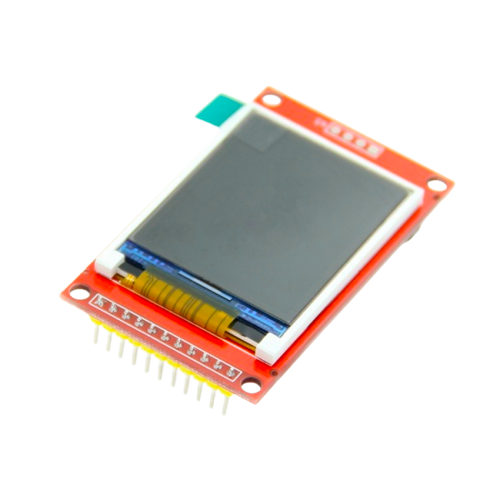
\includegraphics[scale=0.4]{figuras/tftst7735.png}
    \legend{Fonte: Adaptado de \citeonline{tft7735img}.}
    \label{fig:tft7735}
    \centering
\end{figure}

\section{Módulo de acionamento}\label{sec:acionamento}

Um módulo relé, como apresentado na \autoref{fig:rele}, é um componente 
eletrônico utilizado em projetos que envolvem controle 
e automação de dispositivos elétricos. Ele desempenha 
um papel importante ao permitir o controle de circuitos 
de alta potência por meio de sinais de baixa potência.

\begin{figure}[h!]
    \centering
    \caption{Módulo Relé}
    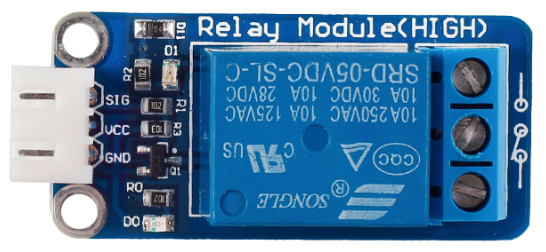
\includegraphics[scale=0.8]{figuras/rele.png}
    \fonte{\citeonline{releimg}}%% Fonte \legend{Fonte: Adaptado de \citeonline{releimg}.}
    \label{fig:rele}
    \centering
\end{figure}

Quando se trata de fechaduras eletrônicas, os módulos relé desempenham um 
papel crucial, facilitando o funcionamento e a segurança do sistema de 
controle de acesso. Geralmente, essas fechaduras 
incluem um mecanismo de trinco que pode ser controlado eletronicamente. 
O módulo relé é utilizado para controlar a ativação e desativação 
desse mecanismo, quando um usuário autorizado fornece uma credencial 
válida (como uma senha, cartão RFID ou impressão digital), o sistema 
eletrônico de controle gera um sinal de baixa potência para acionar 
o módulo relé. O relé fecha seu contato, permitindo a passagem de 
energia para o mecanismo de destravamento da fechadura, liberando 
assim o acesso.

\section{Desenvolvimento do \textit{software}}\label{sec:software}

Para o desenvolvimento do \textit{software}, foi necessário escolher uma plataforma 
de desenvolvimento capaz de programar e gravar códigos nos microcontroladores 
ESP32. Das opções conhecidas eram o Arduino IDE e o PlatformIO. 
Além disso, o desenvolvimento exigiu um estudo aprofundado das 
bibliotecas disponíveis para atender aos requisitos do projeto, 
tais como o reconhecimento facial, transmissão em tempo real de 
imagens em um \textit{display} LCD, implementação de um \textit{timer} e a manipulação 
dos dados de entrada e saída.

\subsection{PlatformIO}\label{sec:platformio}

A plataforma escolhida para esse projeto foi o PlatformIO, 
que é uma alternativa para quem trabalha com dispositivos 
microcontrolados, como o ESP32. Projetado para simplificar o processo 
de desenvolvimento e programação de microcontroladores, o PlatformIO 
oferece diversos recursos e uma abordagem unificada que 
facilita o trabalho com diferentes plataformas de \textit{hardware} e 
ambientes de desenvolvimento.

O PlatformIO destaca-se especialmente ao lidar com o ESP32, 
oferecendo aos desenvolvedores a capacidade de criar suas 
aplicações de forma eficiente, inclusive de maneira remota.
Essa ferramenta foi projetada para funcionar com diversos editores de 
código, como \textit{Visual Studio Code} (VSCode), Atom e CLion,  
permitindo que os desenvolvedores escolha a IDE que melhor 
se adapte às suas preferências. Um ponto forte da ferramenta 
é que a plataforma possui um gerenciador de bibliotecas interno que facilita a 
pesquisa, instalação e atualização direto com o código-fonte, contribuindo 
com a reutilização e organização do código. Além disso, outro ponto foi a 
simplicidade e a rapidez no processo de compilação e carregamento do código 
no ESP32.

Para estabelecer a comunicação com o PlatformIO, tanto para gravação quanto para 
a leitura de dados no ESP32-CAM, a utilização do adaptador ESP32-CAM MB 
(conforme representado na \autoref{fig:adaptadoresp32}) revelou-se necessário. 
Este módulo foi muito importante, pois simplificou a conexão do ESP32-CAM 
com o computador.

\begin{figure}[h!]
    \centering
    \caption{Módulo Adaptador ESP32-CAM MB}
    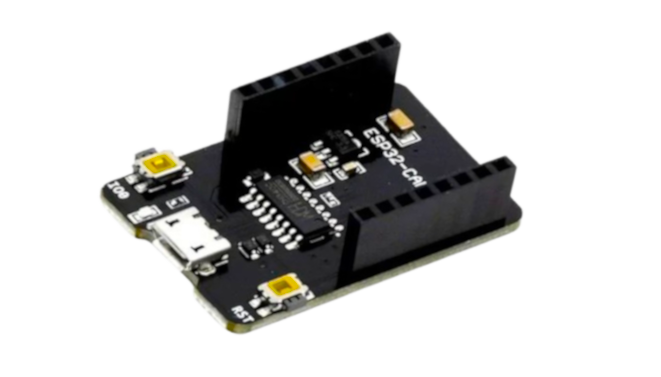
\includegraphics[scale=0.25]{figuras/adaptador_esp32cam.png}
    \legend{Fonte: Adaptado de \citeonline{adaptadoresp32}.}
    \label{fig:adaptadoresp32}
    \centering
\end{figure}

\subsection{Biblioteca ESP-DL}\label{sec:formatacaoTexto}

A biblioteca mais importante nesse projeto foi a \citeonline{espdl}, 
uma ferramenta que disponibiliza Interfaces de Programação de Aplicações 
(APIs) para tarefas como inferência de redes neurais (NN), 
processamento de imagens, operações matemáticas 
e alguns modelos de aprendizado profundo. Essa biblioteca 
contribuiu tanto na implementação da identificação de rostos, 
quanto na execução do processo de reconhecimento facial.

Dentre os recursos disponíveis do ESP-DL, se encontra o 
ESP-Face, componente que fornece funções de detecção e 
reconhecimento facial e também operações de rede neural. 
O método utilizado para detecção facial foi o \textit{face detect} 
(como pode ser visto na \autoref{code:identificacao}) 
e que tem como base o modelo de redes neurais MTMN.

\begin{sourcecode}[htb]
\caption{\label{code:identificacao}Função de detecção facial}
\begin{lstlisting}[frame=single]
#include "fd_forward.h"

box_array_t *run_face_detect(camera_fb_t *fb, dl_matrix3du_t *image_matrix)
{
    fmt2rgb888(fb->buf, fb->len, fb->format, image_matrix->item);
    return face_detect(image_matrix, &mtmn_config);
}    
\end{lstlisting}
\fonte{}
\end{sourcecode}

No contexto do reconhecimento facial, uma vez que um rosto 
humano tenha sido detectado por meio do procedimento 
mencionado anteriormente, é possível realizar uma verificação 
comparando-o com os rostos previamente cadastrados. 
A entrada para esse processo é a imagem original juntamente 
com os resultados obtidos na etapa de detecção facial.

O método de reconhecimento facial, denominado \textit{recognize face}  
(como pode ser visto na \autoref{code:reconhecimento}) 
faz uso do modelo FRMN.

\begin{sourcecode}[htb]
\caption{\label{code:reconhecimento}Função de reconhecimento facial}
\begin{lstlisting}[frame=single]
#include "fr_forward.h"
#define FACE_WIDTH 56
#define FACE_HEIGHT 56
#define MAX_NUMBER_USER 5

int run_face_recognition(face_id_list *id_list, dl_matrix3du_t *image_matrix, box_array_t *net_boxes, int *user_number, bool *enroll_enabled)
{
    dl_matrix3du_t *aligned_face = NULL;
    int matched_id = -1;
    aligned_face = dl_matrix3du_alloc(1, FACE_WIDTH, FACE_HEIGHT, 3);
    if (align_face(net_boxes, image_matrix, aligned_face) == ESP_OK)
    {
        if (*enroll_enabled)
        {
            if (MAX_NUMBER_USER == *user_number)
			    {
				    dl_matrix3du_free(aligned_face);
				    return matched_id;
			    }
            else
            {
                int8_t number_file = enroll_face(id_list, aligned_face);
            }
        }
        else
        {
            matched_id = recognize_face(id_list, aligned_face);
        }
    }
    dl_matrix3du_free(aligned_face);
    return matched_id;
}
\end{lstlisting}
\fonte{}
\end{sourcecode}

\subsection{Fluxo de telas}\label{sec:telas}

Os recursos gráficos fornecidos pelo \textit{display} LCD melhorou de 
forma substancial a usabilidade da aplicação. Nesse contexto, a elaboração 
do fluxo de telas se tornou indispensável para proporcionar aos usuários 
uma experiência eficiente. Todos os fluxos foram planejados e 
projetados com o objetivo de guiar o usuário por meio 
de diferentes interações e funcionalidades.

A criação dos fluxos de telas foi realizada por meio do \textit{software} GIMP 
(\textit{GNU Image Manipulation Program} ou Programa de Manipulação 
de Imagem do GNU). Trata-se de uma aplicação de código aberto 
dedicada à criação e edição de imagens, conforme ilustrado 
na \autoref{fig:gimp}.

\begin{figure}[h!]
    \centering
    \caption{Criação e edição da tela do menu}
    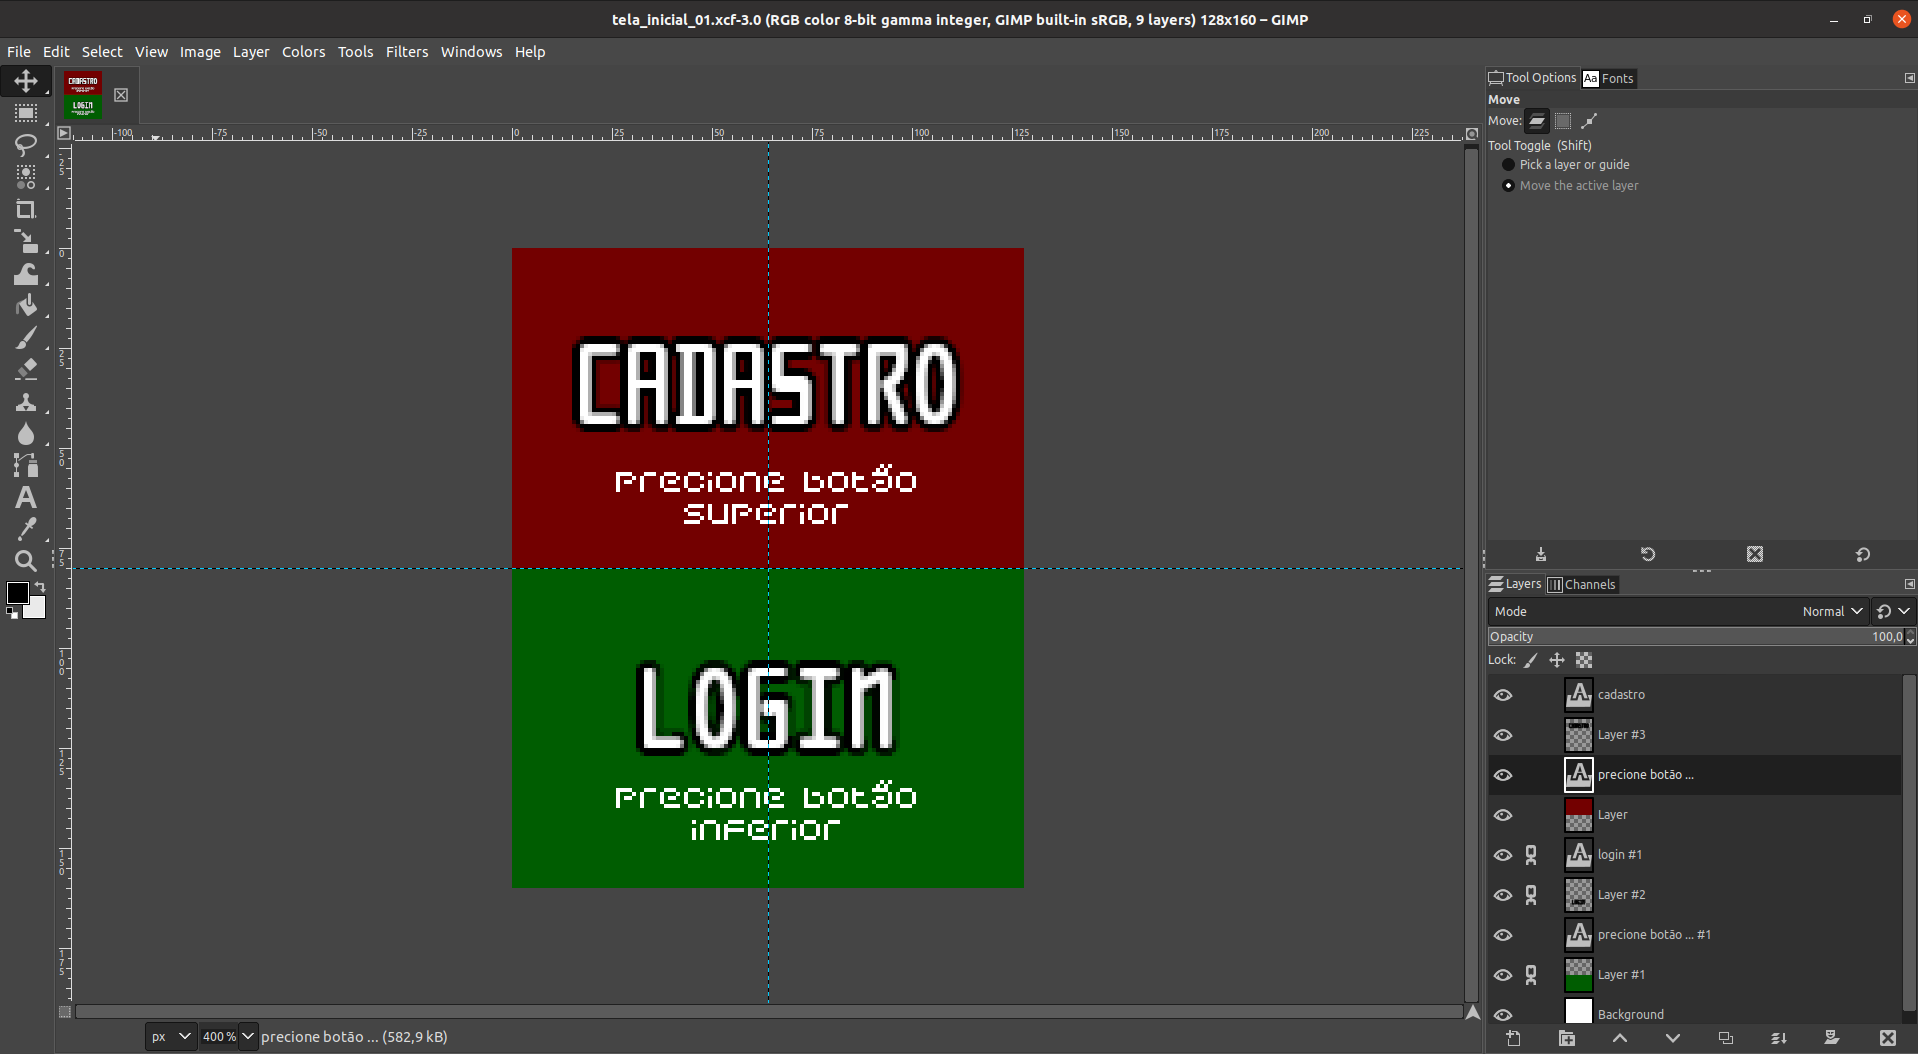
\includegraphics[scale=0.2]{figuras/gimp.png}
    \legend{}
    \label{fig:gimp}
    \centering
\end{figure}

E para exibir as imagens do fluxo de telas no \textit{Display} 
LCD, optou-se pelo uso da biblioteca \textit{TFT eFEX}, 
conforme ilustrado no trecho de código apresentado 
na \autoref{code:tft}.

\begin{sourcecode}[htb]
\caption{\label{code:tft}Função de exibição do menu}
\begin{lstlisting}[frame=single]
#include "TFT_eFEX.h"
TFT_eFEX fex = TFT_eFEX(&tft);

void display_menu()
{
    fex.drawJpgFile(SPIFFS, "/_initial.jpeg", 0, 0);
    delay(200); // Debounce
} 
\end{lstlisting}
\fonte{}
\end{sourcecode}

\section{Desenvolvimento do protótipo}\label{sec:prototipo}

Para o desenvolvimento do protótipo, utilizou-se o 
\textit{software KiCad} (\autoref{fig:kicad}), uma aplicação de código aberto destinada a 
projetos eletrônicos. Sua finalidade é simplificar a criação 
de layouts e a conversão destes para placas de circuito 
impresso (PCB). O \textit{KiCad} apresenta ferramentas 
abrangentes para a elaboração da estrutura do produto, 
criação de arte final e visualizações tridimensionais da PCB e 
seus componentes. Por meio dele, foi criado um diagrama elétrico  
detalhado, conforme ilustrado na \autoref{fig:circuito}. Este diagrama 
foi construído com base em um circuito previamente montado e testado em 
uma placa de prototipagem ou \textit{protoboard}. 

\begin{figure}[h!]
    \centering
    \caption{Menu KiCad}
    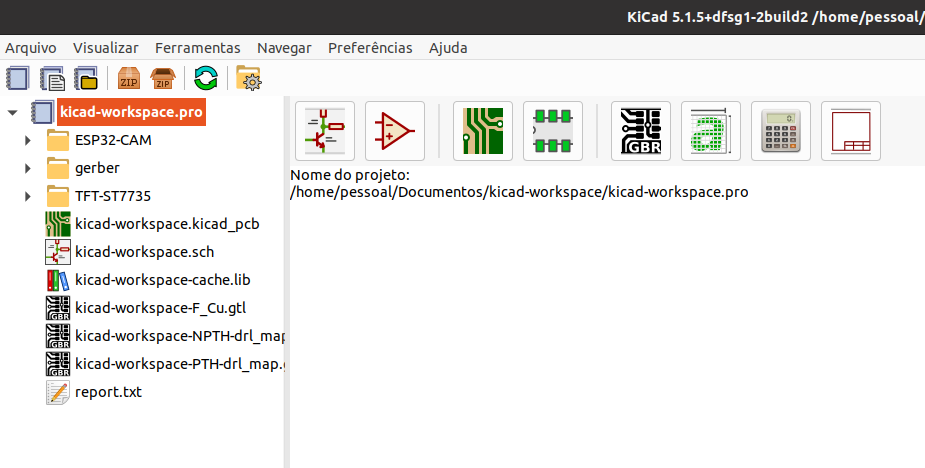
\includegraphics[scale=0.4]{figuras/kicad.png}
    \fonte{}%% Fonte
    \label{fig:kicad}
    \centering
\end{figure}

\begin{figure}[h!]
    \centering
    \caption{Diagrama elétrico do protótipo}
    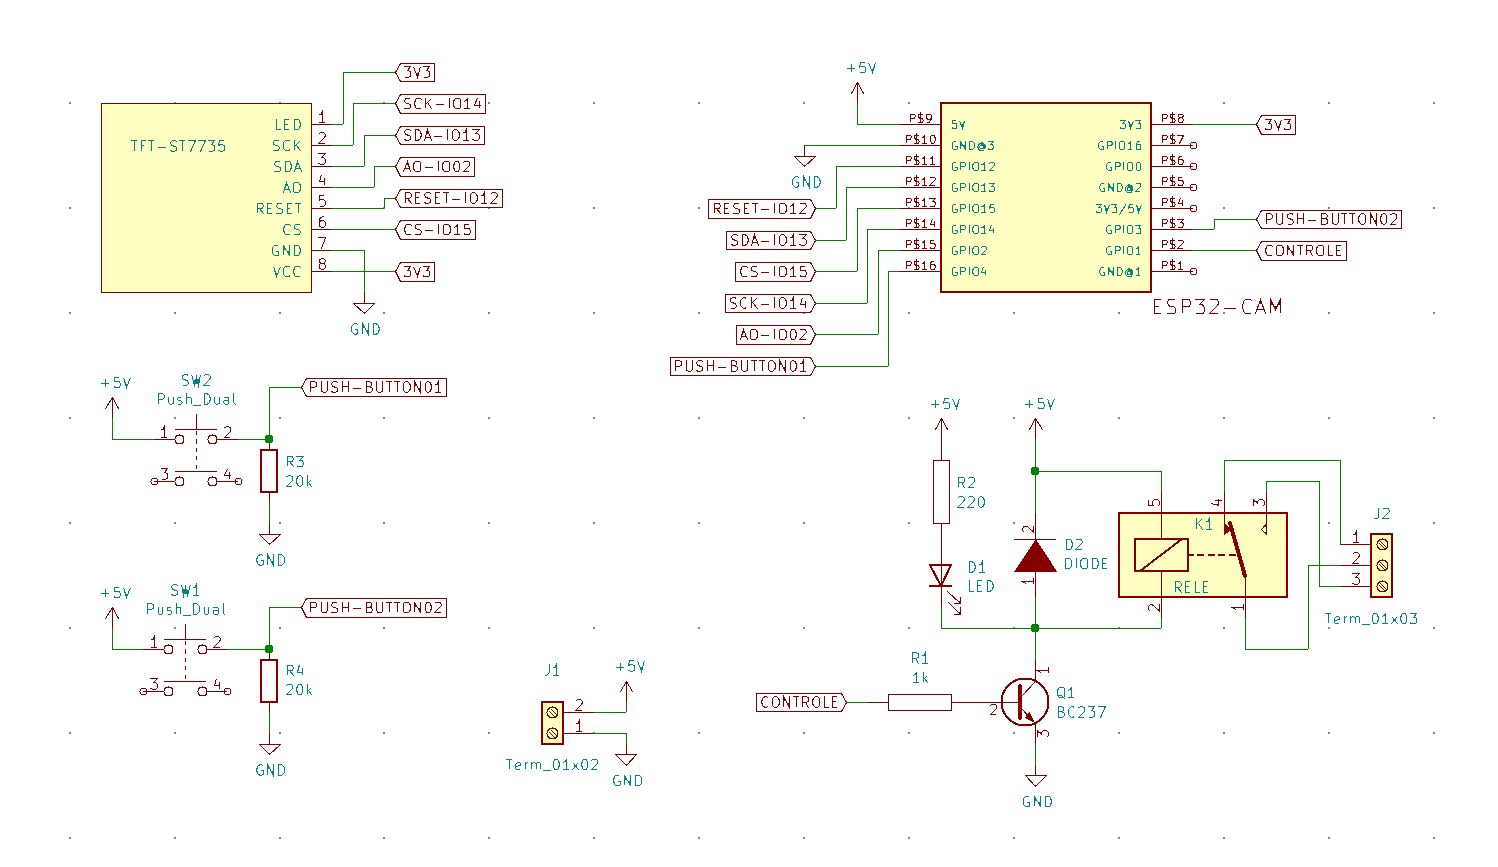
\includegraphics[scale=0.3]{figuras/circuito_completo.png}
    \fonte{}%% Fonte
    \label{fig:circuito}
    \centering
\end{figure}

O diagrama elétrico do protótipo divide o circuito em quatro blocos 
principais: o ESP32-CAM, o TFT ST7735, o módulo de relé e o módulo 
de botões (\textit{push button}). O bloco principal, que é o ESP32-CAM, 
possui 16 pinos de entrada/saída (GPIOs), como representado na 
\autoref{fig:diagramaesp} e desempenha o papel de controle e 
coordenação do sistema como um todo. Dos 16 pinos disponíveis, 
7 são dedicados ao \textit{display} TFT (GPIOs 2, 12, 13, 14 e 15), 2 são 
reservados para os botões (GPIOs 4 e 3) e 1 pino é utilizado 
como saída para controlar o módulo do relé (GPIO 1).

Importante mencionar que algumas GPIOs têm funções específicas. 
Por exemplo, a GPIO 16 permanece em nível lógico alto e é utilizada 
para habilitar a memória PSRAM. Além disso, a GPIO 0 é designada como 
\textit{clock} da câmera e não pode ser realocada para outras finalidades, 
uma vez que isso afetaria o funcionamento adequado da captura de 
imagens. Essas atribuições de GPIOs foram cuidadosamente 
planejadas para garantir o correto funcionamento de 
cada componente do protótipo. 

\begin{figure}[h!]
    \centering
    \caption{Diagrama elétrico do ESP32-CAM}
    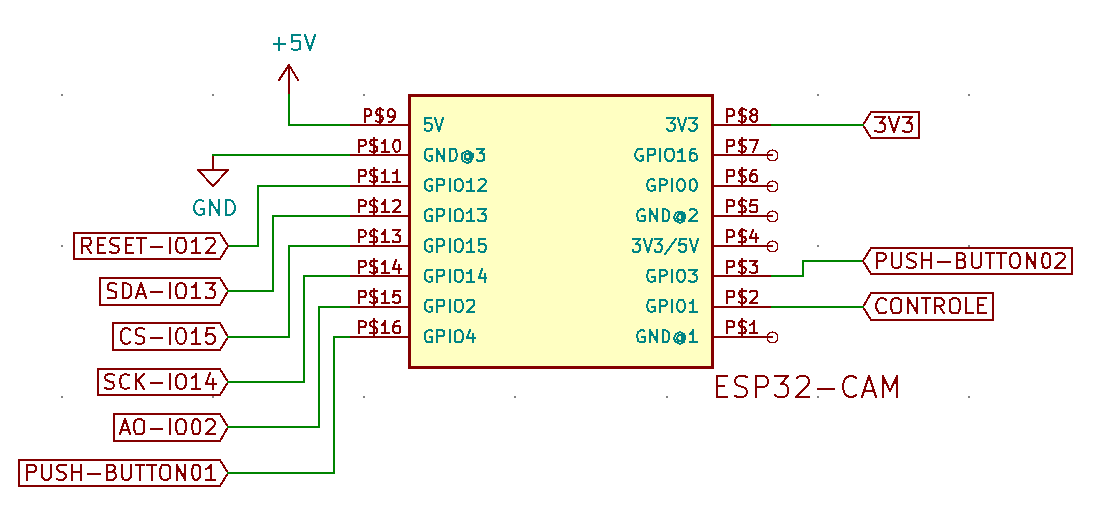
\includegraphics[scale=0.3]{figuras/modulo_esp.png}
    \fonte{}%% Fonte
    \label{fig:diagramaesp}
    \centering
\end{figure}

O segundo bloco corresponde ao controlador ST7735 (\autoref{fig:diagramatft}), 
um componente projetado para o gerenciamento de \textit{displays} TFT de tamanho 
reduzido e com capacidade de exibir cores. A principal função desse 
controlador é administrar a apresentação de informações na tela, 
permitindo a criação de gráficos e a exibição de texto colorido.

A tela em si é composta por uma matriz de \textit{pixels} coloridos, em que 
cada \textit{pixel} é formado por subpixels nas cores vermelha, verde e azul 
(RGB), possibilitando a exibição de uma vasta gama de cores. Os pinos 
SCK (\textit{Serial Clock}), SDA e CS (\textit{Chip Select}) são utilizados para a 
comunicação serial com o microcontrolador. Por sua vez, o pino de 
\textit{reset} é designado para reiniciar o \textit{display} em caso de falhas ou erros.

Adicionalmente, o pino A0 indica 
se os dados transmitidos se referem a comandos de controle (estado \textit{LOW}) 
ou a dados de \textit{pixel} (estado \textit{HIGH}), desempenhando um papel crucial no 
funcionamento adequado do controlador ST7735.

\begin{figure}[h!]
    \centering
    \caption{Diagrama elétrico do \textit{Display} TFT}
    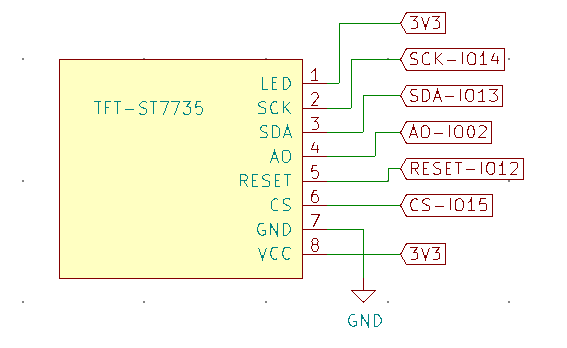
\includegraphics[scale=0.36]{figuras/modulo_tft.png}
    \fonte{}%% Fonte
    \label{fig:diagramatft}
    \centering
\end{figure}

O bloco que compreende os botões é importante na 
interatividade do projeto, pois permite a seleção de itens no menu 
e a inserção dos valores da senha. A estrutura dos botões é 
ilustrada no circuito apresentado na \autoref{fig:diagramabotoes}, e 
cada botão é capaz de enviar um sinal de nível lógico baixo quando não 
pressionado e de nível lógico alto quando acionado, transmitindo esses 
sinais ao microcontrolador.

Devido a mudança de estado do botões ao alterar o sinal elétrico conforme 
são pressionados ou soltos, permite ao microcontrolador reconhecer as ações 
do usuário, possibilitando a navegação no aplicativo de forma eficiente 
e prática. Isso faz com que esses componentes contribuam significativamente 
com a interatividade do protótipo e a experiência do usuário.

\begin{figure}[h!]
    \centering
    \caption{Diagrama elétrico dos botões}
    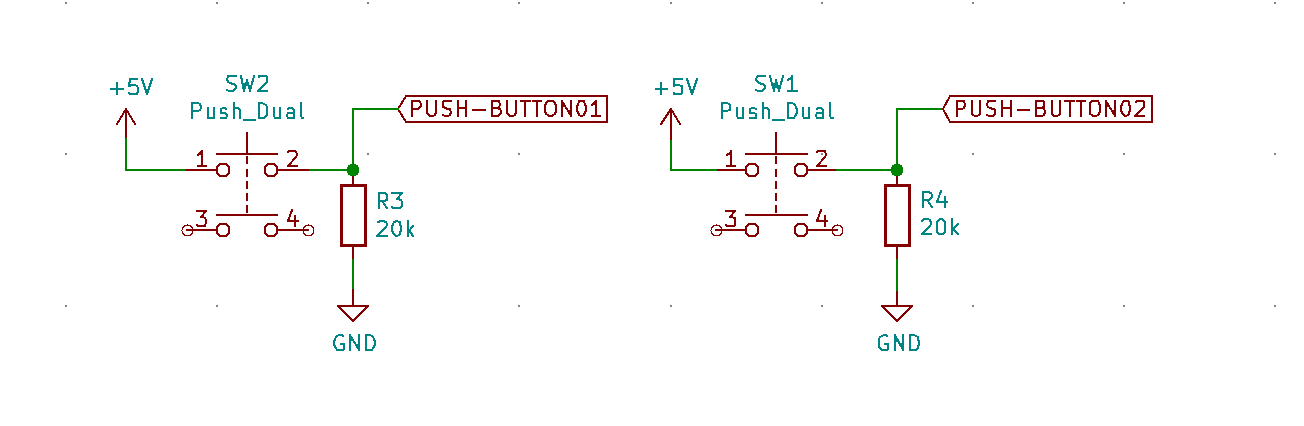
\includegraphics[scale=0.25]{figuras/modulo_push.png}
    \fonte{}%% Fonte
    \label{fig:diagramabotoes}
    \centering
\end{figure}

O módulo de relé, conforme apresentado na (\autoref{fig:diagramarele}), 
consiste em um circuito que viabiliza que um microcontrolador 
envie um sinal de baixa potência para a base de um transistor. A conexão do 
coletor do transistor à bobina do relé viabiliza o seu acionamento 
quando o transistor entra em estado de saturação. Isso, por sua vez, permite que o ESP32 
controle dispositivos de alta potência por meio de sinais de baixa potência. 
O diodo em paralelo ao relé, também conhecido como diodo de roda 
livre, desempenha o papel de proteger o circuito de picos ou sobretensão reversa.

\begin{figure}[h!]
    \centering
    \caption{Diagrama elétrico do módulo relé}
    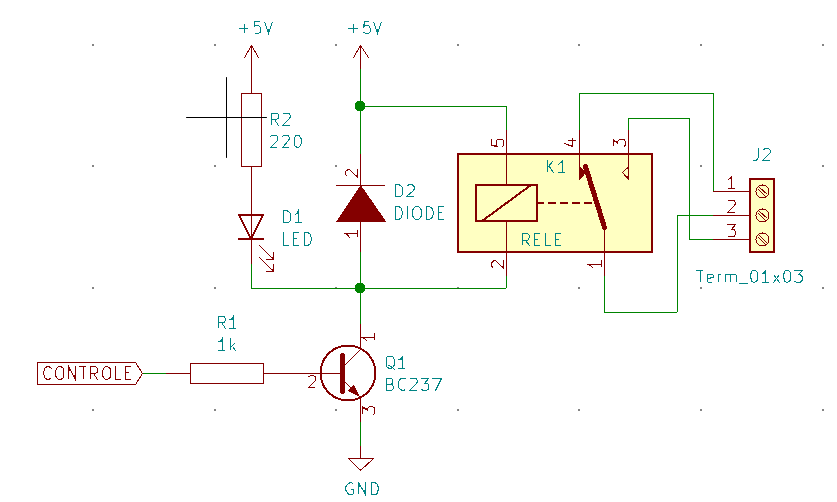
\includegraphics[scale=0.2]{figuras/modulo_rele_esquema.png}
    \fonte{}%% Fonte
    \label{fig:diagramarele}
    \centering
\end{figure}

A escolha dos conectores do tipo borne KRE para as conexões de entrada 
e saída do circuito se justifica pela praticidade e segurança que 
eles oferecem, devido ao seu encaixe lateral que simplifica a 
conexão com fios e outros módulos eletrônicos.